%% ----------------------------------------------------------------------
%% START OF FILE
%% ----------------------------------------------------------------------

\chapter{系统测试与结果分析}
\label{cha:exp_analysis}

\section{测试平台}
\label{sec:exp_platform}

操作系统 Microsoft Windows Server 2008 R2

机械硬盘 250GB seagate st9250320as

固态硬盘 120GB crucial ct120m500ssd1

驱动程序开发工具 Microsoft Windows Driver Kit 7600.1

应用程序开发工具 Microsoft Visual Studio 2008

\section{测试方法}
\label{sec:exp_method}

本缓存系统在Windows平台下实现,整个系统测试工作包括了系统正确性验证和系统性能测试两个方面的评估。

\subsection{系统正确性验证}

正确性验证使用了Windows自带的chkdsk工具,该工具能够检测存储卷保存的文件系统是否存在问题。测试之前需要保证被测试的缓存卷本身不存在问题,最好的方法是使用系统自带的分区管理工具建立新存储卷用于测试。

正确性验证的步骤为:
\begin{enumerate}
\item 加载缓存驱动程序。
\item 开启对某个存储卷的缓存。
\item 使用性能测试工具测试被缓存的存储卷读写性能。
\item 停止存储卷的缓存。
\item 卸载缓存驱动程序。
\item 使用chkdsk检测被缓存的存储卷。
\end{enumerate}

如果最后一步chkdsk命令的检测没有出现问题,则说明缓存系统通过了正确性的验证。

\subsection{系统性能测试}

\subsubsection{性能测试工具FIO}
FIO是一款广泛使用的基于GPLv2协议的存储器性能评测工具,主要用于测试存储设备的性能和压力上限。除了存储设备,FIO还提供了针对CPU和NIC的IO性能测试功能。FIO支持13种不同的IO引擎,可以通过多线程或多进程模拟各种IO操作。作为一款开源工具,FIO支持几乎所有的操作系统平台:Linux,FreeBSD,NetBSD,OS X,OpenSolaris,AIX以及Windows。

FIO只提供了命令行界面的用户交互方式。由于其提供了丰富的可调整的参数,FIO的可定制性非常强,可以根据测试者的意图进行多种模式的测试。本系统测试工作也只使用了其中的一小部分参数。

\subsubsection{参数说明}

以下逐一介绍论文系统测试中所用到的各FIO选项,并对其参数加以说明。

\begin{lstlisting}
filename=\\\\.\\C:
\end{lstlisting}

filename参数指定了需要进行测试的设备文件。本论文实现的缓存系统以存储卷为单位,Windows操作系统只有将存储卷映射到某个的盘符(C、D、E……)后,才可进行访问。因此,对FIO来说要测试的存储设备指的就是某个盘符所映射的存储卷。

\begin{lstlisting}
size=2000MB
\end{lstlisting}

size参数指定待测试存储设备的空间大小,本论文测试的机械硬盘存储卷大小为2000MB。一般来说,缓存大小设定为存储空间大小的5\%-15\%,缓存系统对系统IO性能提升的贡献最为明显,存在也更有意义。因此,论文测试中将缓存卷的大小设定为200MB。固态硬盘上的缓存卷可使用系统自带的存储卷管理程序划分。

\begin{lstlisting}
iodepth=8
\end{lstlisting}

iodepth参数用以设定测试中最大的并发IO请求个数。应用程序通常使用同步和异步两种方式访问存储设备。以同步方式访问设备时,下一个IO请求要在上一个完成后才可进行,因此iodepth总是为1;异步方式访问,每次提交一批IO请求然后等这一批请求的完成,这样做可以减少交互的次数,让设备有机会合并IO请求以及进行内部的并行处理。在多进程的操作系统内,绝大多数情况下设备访问的iodepth都会大于1。

\begin{lstlisting}
numjobs=4
\end{lstlisting}

numjobs参数设定了同时进行的负载个数,每个线程能产生一个负载进行测试。numjobs指定了FIO同时启动的测试线程数目。

\begin{lstlisting}
blocksize=[4k, 16k, 64k]
\end{lstlisting}

blocksize参数指定了测试时每个IO请求的大小,即每次读写的存储块大小,默认值为4KB。本论文分别使用了4KB,16KB,64KB三种不同大小进行测试,以模拟不同应用场景下应用程序对于存储设备的读写请求,同时还可以评估设定的可变长缓存块大小对于缓存系统性能的影响。

\begin{lstlisting}
rw=[randrw, randread, randwrite]
\end{lstlisting}

rw参数设定每次测试所产生的读写类型。FIO提供了顺序读、顺序写、混合顺序读写、随机读、随机写、混合随机读写六种读写类型,每次测试只能选择其中一种。任何缓存系统应对顺序读写性能提升的贡献效果都非常有限,因此本论文不进行顺序读写的测试,只测试随机读、随机写和混合随机读写三种读写类型。

\begin{lstlisting}
runtime=1000
\end{lstlisting}

runtime参数控制FIO运行多长时间后退出执行,并给出测试结果,单位是秒。如果运行时间太短,测试结果受系统内其他进程影响,波动较大。经过多次实验,测试时间长为1000秒时性能趋于稳定,此时的测试结果最有说服力。

\begin{lstlisting}
random_distribution=zipf:1.2
\end{lstlisting}

FIO提供random\_distribution参数配置测试中访问存储设备的位置分布类型。通过设置该参数,可以使某部分的访问概率比其他部分的大,而并非平均分散到各处,从而获得系统存在热数据的访问效果。默认参数下,测试中设备的访问位置完全随机分布,此时测试出的缓存性能无法体现出真实情况下热数据被频繁访问的效果,缓存命中率也不具备说服力。而本论文的测试中,使用了齐夫分布这种概率分布模型,齐夫分布是一种最常见的模拟热数据访问的概率模型,参数为1.2。

\section{测试结果}
\label{sec:exp_results}

经chkdsk工具测试,结果表明论文实现的缓存系统,正确性方面没有任何问题,下面主要对缓存系统的性能测试结果加以分析。

论文实现的缓存系统可运行于写穿(Write Through)和写回(Write Back)两种模式,每种模式下需要进行随机读、随机写和混合随机读写三种类型的测试。

\subsection{缓存命中率}

\begin{table}[H]
\centering
\caption{写回、写穿两种模式下的缓存命中率}
\begin{tabular}{|c|c|c|c|}
\hline
\diagbox{模式}{测试类型} & 随机读 & 随机写 & 混合随机读写 \\ 
\hline 写穿模式 & 70.27\% & 70.75\% & 70.61\% \\ 
\hline 写回模式 & 76.29\% & 76.43\% & 73.64\% \\ 
\hline 
\end{tabular} 
\label{tab:cache-hit-rate}
\end{table}

从上表可以看出,写回模式下,缓存命的中率略高于写穿模式。这是因为,不定期的回写队列刷新操作,延长了数据在缓存中的停留,一定程度上提升了命中率。

\subsection{写穿(Write Through)模式下的测试结果}

\subsubsection{随机读速度测试}

\begin{table}[H]
\centering
\caption{随机读速度(KB/s,写穿法)}
\begin{tabular}{|c|c|c|c|}
\hline
\diagbox{块大小(KB)}{存储介质} & HDD & SSD & HDD with SSD Cache \\ 
\hline 4 & 417 & 19264 & 2063 \\ 
\hline 16 & 1651 & 59735 & 6319 \\ 
\hline 64 & 5810 & 142304 & 13203 \\ 
\hline 
\end{tabular} 
\label{tab:wt-rand-read-test}
\end{table}

写穿模式下,SSD缓存带来了2.3-4.9倍的HDD随机读性能提升。

\subsubsection{随机写速度测试}

\begin{table}[H]
\centering
\caption{随机写速度(KB/s,写穿法)}
\begin{tabular}{|c|c|c|c|}
\hline
\diagbox{块大小(KB)}{存储介质} & HDD & SSD & HDD with SSD Cache \\ 
\hline 4 & 1283 & 18620 & 1155 \\ 
\hline 16 & 5043 & 40634 & 4768 \\ 
\hline 64 & 16346 & 41615 & 15490 \\ 
\hline 
\end{tabular} 
\label{tab:wt-rand-write-test}
\end{table}

写穿模式下,由于没有缓存写操作,HDD的随机写性能略差于无缓存情况下的写性能。

\subsubsection{随机读写:读速度测试}

\begin{table}[H]
\centering
\caption{随机读写-读速度(KB/s,写穿法)}
\begin{tabular}{|c|c|c|c|}
\hline
\diagbox{块大小(KB)}{存储介质} & HDD & SSD & HDD with SSD Cache \\ 
\hline 4 & 420 & 14693 & 1590 \\ 
\hline 16 & 1657 & 46650 & 5327 \\ 
\hline 64 & 5598 & 105242 & 11929 \\ 
\hline 
\end{tabular} 
\label{tab:wt-randrw-read-test}
\end{table}

写穿模式下进行随机读写测试,SSD缓存带来了2.3-4.9倍的HDD随机读性能提升。

\subsubsection{随机读写:写速度测试}

\begin{table}[H]
\centering
\caption{随机读写-写速度(KB/s,写穿法)}
\begin{tabular}{|c|c|c|c|}
\hline
\diagbox{块大小(KB)}{存储介质} & HDD & SSD & HDD with SSD Cache \\ 
\hline 4 & 45 & 1688 & 181 \\ 
\hline 16 & 180 & 5427 & 616 \\ 
\hline 64 & 599 & 11925 & 1371 \\ 
\hline 
\end{tabular} 
\label{tab:wt-randrw-write-test}
\end{table}

写穿模式下进行随机读写测试,SSD缓存带来了2.4-4.0倍的HDD随机写性能提升。
理论上讲,工作在写穿模式下的缓存无法带来写的性能提升,上面的‘随机写速度’的测试结果也说明了这点。之所以混合随机读写测试出现了与之相悖的写性能提升效果,是因为混合随机读写模式下,读写任务队列里,间插于写请求中一部分读请求会命中于SSD缓存中。这在一定程度上降低了机械硬盘的读写负载,同时也造就了随机写性能的相对提升。

\subsection{写回(Write Back)策略时的测试结果}

\subsubsection{随机读速度测试}

\begin{table}[H]
\centering
\caption{随机读速度(KB/s,写回法)}
\begin{tabular}{|c|c|c|c|}
\hline
\diagbox{块大小(KB)}{存储介质} & HDD & SSD & HDD with SSD Cache \\ 
\hline 4 & 417 & 19264 & 2970 \\ 
\hline 16 & 1651 & 59735 & 9821 \\ 
\hline 64 & 5810 & 142304 & 32857 \\ 
\hline 
\end{tabular} 
\label{tab:wb-rand-read-test}
\end{table}

写回模式下,SSD缓存带来了5.6-7.1倍的HDD随机读性能提升。

\subsubsection{随机写速度测试}

\begin{table}[H]
\centering
\caption{随机写速度(KB/s,写回法)}
\begin{tabular}{|c|c|c|c|}
\hline
\diagbox{块大小(KB)}{存储介质} & HDD & SSD & HDD with SSD Cache \\ 
\hline 4 & 1283 & 18620 & 3459 \\ 
\hline 16 & 5043 & 40634 & 8697 \\ 
\hline 64 & 16346 & 41615 & 21794 \\ 
\hline 
\end{tabular} 
\label{tab:wb-rand-write-test}
\end{table}

写回模式下,SSD缓存带来了1.3-2.6倍的HDD随机写性能提升。

\subsubsection{随机读写:读速度测试}

\begin{table}[H]
\centering
\caption{随机读写-读速度(KB/s,写回法)}
\begin{tabular}{|c|c|c|c|}
\hline
\diagbox{块大小(KB)}{存储介质} & HDD & SSD & HDD with SSD Cache \\ 
\hline 4 & 420 & 14693 & 2725 \\ 
\hline 16 & 1657 & 46650 & 8693 \\ 
\hline 64 & 5598 & 105242 & 27696 \\ 
\hline 
\end{tabular} 
\label{tab:wb-randrw-read-test}
\end{table}

写回模式下进行随机读写测试,SSD缓存带来了4.9-6.4倍的HDD随机读性能提升。

\subsubsection{随机读写:写速度测试}

\begin{table}[H]
\centering
\caption{随机读写-写速度(KB/s,写回法)}
\begin{tabular}{|c|c|c|c|}
\hline
\diagbox{块大小(KB)}{存储介质} & HDD & SSD & HDD with SSD Cache \\ 
\hline 4 & 45 & 1688 & 309 \\ 
\hline 16 & 180 & 5427 & 985 \\ 
\hline 64 & 599 & 11925 & 3221 \\ 
\hline 
\end{tabular} 
\label{tab:wb-randrw-write-test}
\end{table}

写回模式下进行随机读写测试,SSD缓存带来了5.3-6.8倍的HDD随机写性能提升。

\section{结果讨论}
\label{sec:results_and_comparation}

\subsection{HDD性能提升比例}

\begin{figure}[H]
\centering
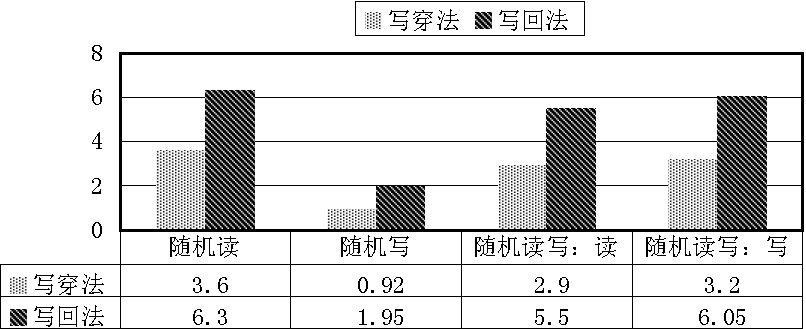
\includegraphics[width=0.9\linewidth]{./graph/enhance-rate}
\caption{读写性能提升比例比较}
\label{fig:enhance-rate}
\end{figure}

从图\ref{fig:enhance-rate}可以看出,缓存系统的存在从一定程度带来了HDD随机读、随机写的性能提升。相较于写穿法,写回法对存储系统的读写性能提升比例更为明显。

\subsection{与商业软件比较}

FancyCache是一款使用SSD作为缓存提升存储系统性能的商业软件。FancyCache可以将系统内存或SSD空间设置成机械硬盘的缓存。该软件的特点是,能够将从机械硬盘中读取的数据存入系统内存或闪存,使系统在下次访问该数据时可以很快从内存读取,避免再次读取速度较慢的硬盘,从而突破硬盘瓶颈,提升系统性能。FancyCache还能够通过特殊方式,识别并使用32位操作系统无法识别出的物理内存,解决32位Windows操作系统无法完全使用4G或更多内存的问题。

为了说明本论文实现的缓存系统与缓存软件FancyCache对系统性能提升的差距,在系统的实验阶段,论文还测试了使用FancyCache缓存软件时的HDD读写性能提升。由于通过上节的测试可以得出本论文实现的缓存系统运行于回写模式时,对HDD的随机读写性能提升最为明显。且FancyCache的软件缓存同样运行于写回模式。因此,本节会使用运行于写回模式时的测试数据与FancyCache软件进行比较。

\begin{table}[H]
\centering
\caption{随机读速度比较(KB/s)}
\begin{tabular}{|c|c|c|}
\hline
\diagbox{块大小(KB)}{缓存系统} & 本论文的 & FancyCache \\ 
\hline 4  & 2970 & 2508 \\ 
\hline 16 & 9821 & 10254 \\ 
\hline 64 & 32857 & 51833 \\ 
\hline 
\end{tabular} 
\label{tab:wb-rand-read-comp}
\end{table}

从随机读测试的结果可以看出,IO请求的大小为4KB时,本论文实现的缓存系统性能优于FancyCache;当IO请求比较大时,FancyCache的效果更为明显,这是因为论文实现的缓存系统的缓存块大小为4KB,读写请求大于4KB时会将一个读写请求切分为多个处理,影响了系统的性能。

\begin{table}[H]
\centering
\caption{随机写速度比较(KB/s)}
\begin{tabular}{|c|c|c|}
\hline
\diagbox{块大小(KB)}{缓存系统} & 本论文的 & FancyCache \\ 
\hline 4  & 2970 & 3021 \\ 
\hline 16 & 9821 & 9982 \\ 
\hline 64 & 32857 & 32258 \\ 
\hline 
\end{tabular} 
\label{tab:wb-rand-write-comp}
\end{table}

进行随机写测试,IO请求的大小为4KB和16KB时,FancyCache的性能优于本论文实现的缓存系统,但差距不大;IO请求的大小为64KB时,本论文实现的缓存系统性能略优于FancyCache。

%% ----------------------------------------------------------------------
%%% END OF FILE
%% ----------------------------------------------------------------------
